\documentclass{article}
\usepackage[margin=1in]{geometry}
\usepackage{graphicx}
\usepackage{float}
\usepackage{amsmath}
\usepackage{enumitem}
\usepackage{booktabs}

\title{Open-Storm.org Control Test Cases}

\begin{document}
\maketitle
\tableofcontents
\section{Single Tank}

\section{Tanks in Series}
\subsection{Study Area Map}

\begin{figure}[H]
  \centering
  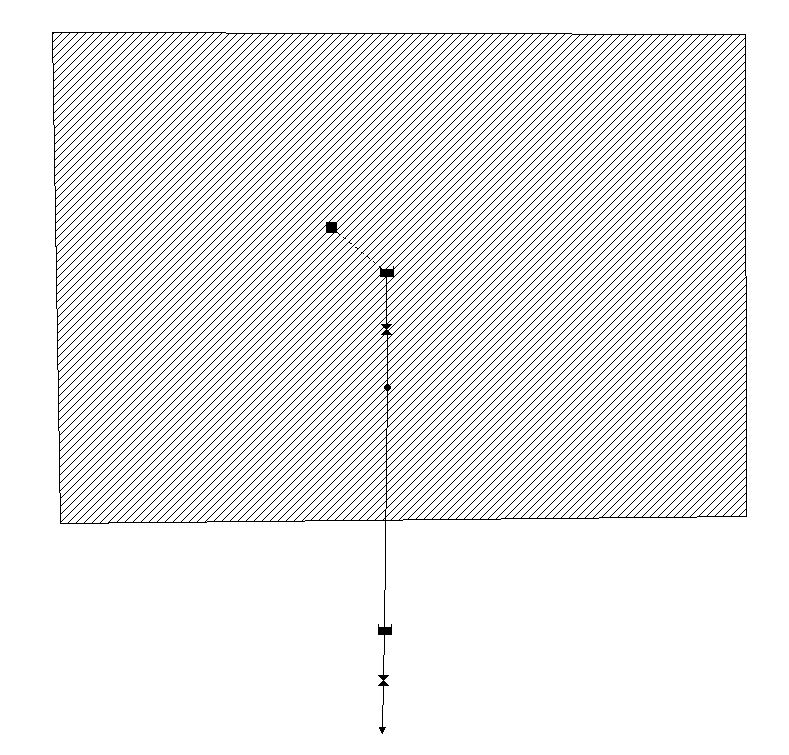
\includegraphics[width = 0.5\textwidth]{series.JPG}
\end{figure}

\subsection{Site Summary}
\begin{table}[H]
\centering
\label{my-label}
\begin{tabular}{lll}
Element Label & Nature         & Specifications   \\
S5            & Detention Pond & Max Height = 3.65m  \\
  S7            & Detention Pond & Max Height = 3.65m \\
  C8 &Orifice & Node : S5\\
  R2 &Orifice & Node : S7\\
\end{tabular}
\caption{Table summarizing controllable storm water assets}
\end{table}
[Insert site summary]
\subsection{Uncontrolled Response}
\begin{figure}[H]
  \centering
  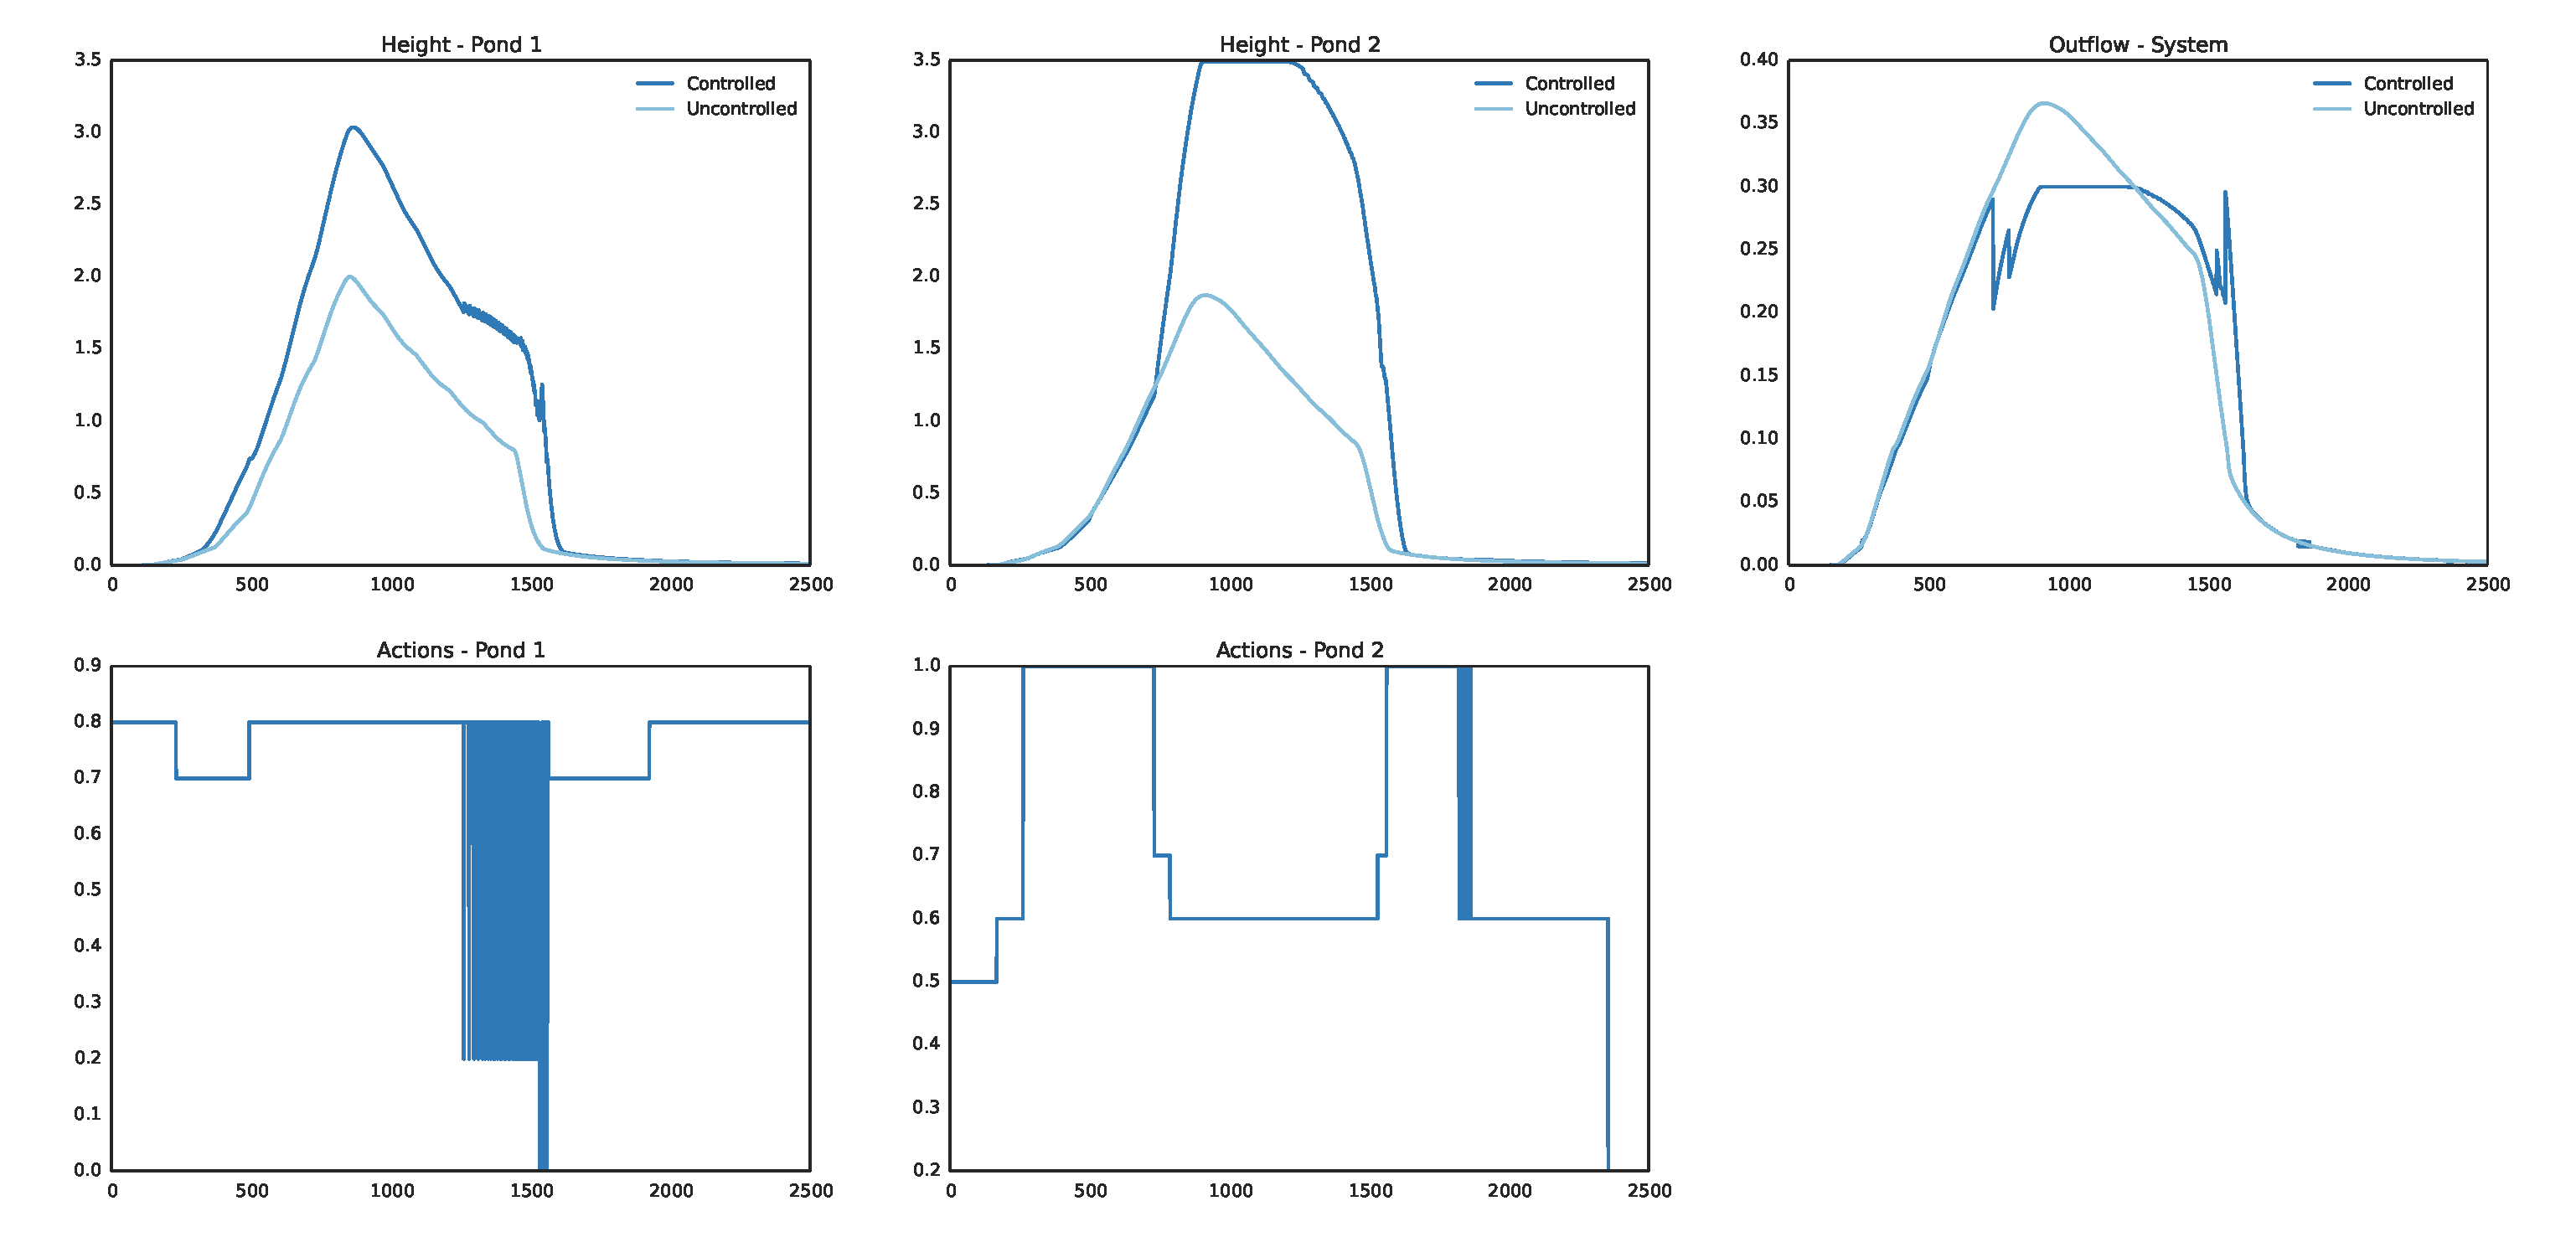
\includegraphics[width = 0.9\textwidth]{figure_1.eps}
\end{figure}


\section{Tanks in Parallel}

\subsection{Study Area Map}

\begin{figure}[H]
  \centering
  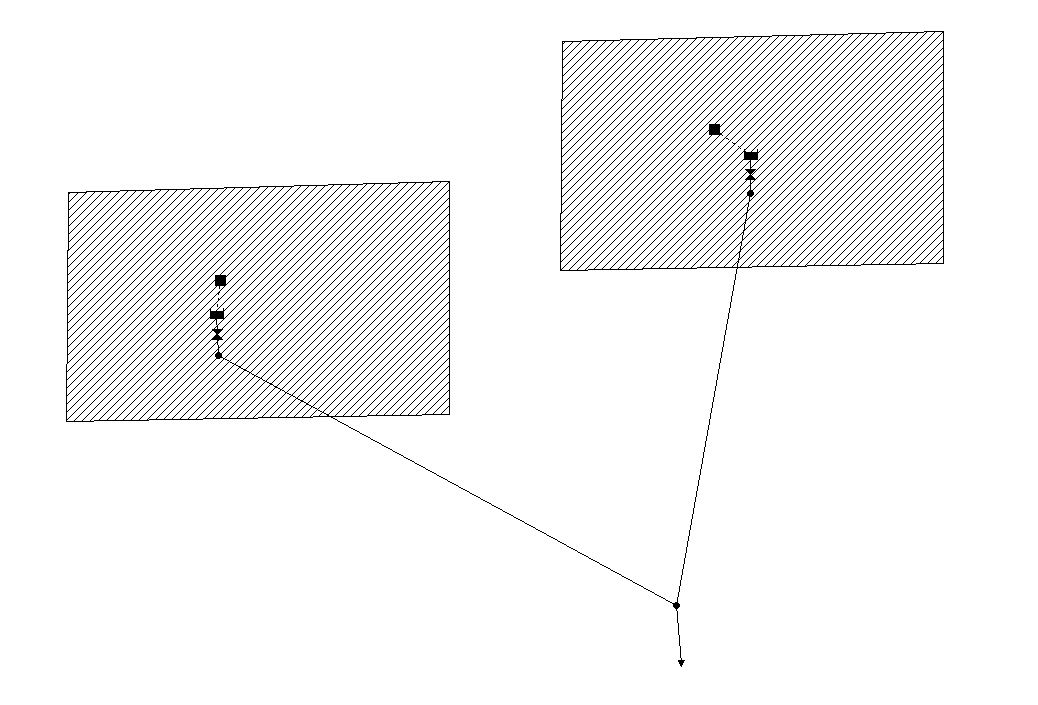
\includegraphics[width = 0.5\textwidth]{parallel.JPG}
\end{figure}

\subsection{Site Summary}
\begin{table}[H]
\centering
\label{my-label}
\begin{tabular}{lll}
Element Label & Nature         & Specifications   \\
S1            & Detention Pond & Max Height = 3.6m  \\
  S2            & Detention Pond & Max Height = 3.6m  \\
  OR1 & Orifice & Node:S1\\
  OR2 & Orifice & Node:S2
\end{tabular}
\caption{Table summarizing controllable storm water assets}
\end{table}
[Insert site summary]
\subsection{Uncontrolled Response}
\begin{figure}[H]
  \centering
  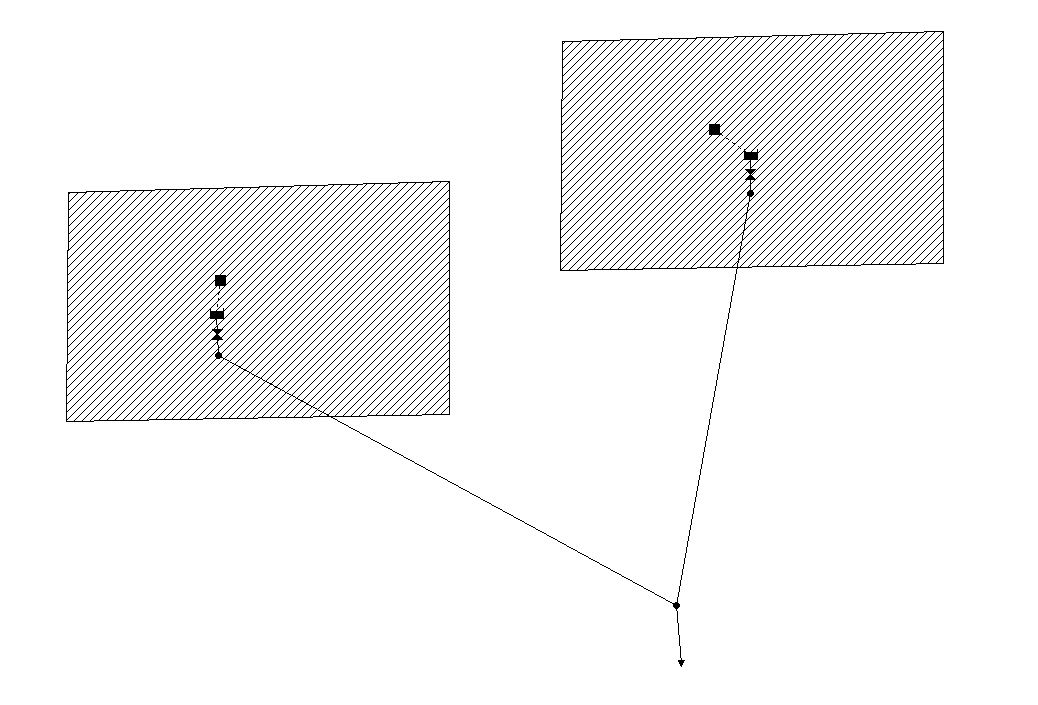
\includegraphics[width = 0.9\textwidth]{parallel.eps}
\end{figure}


\section{Combination of Series and Parallel}

\subsection{Study Area Map}

\begin{figure}[H]
  \centering
  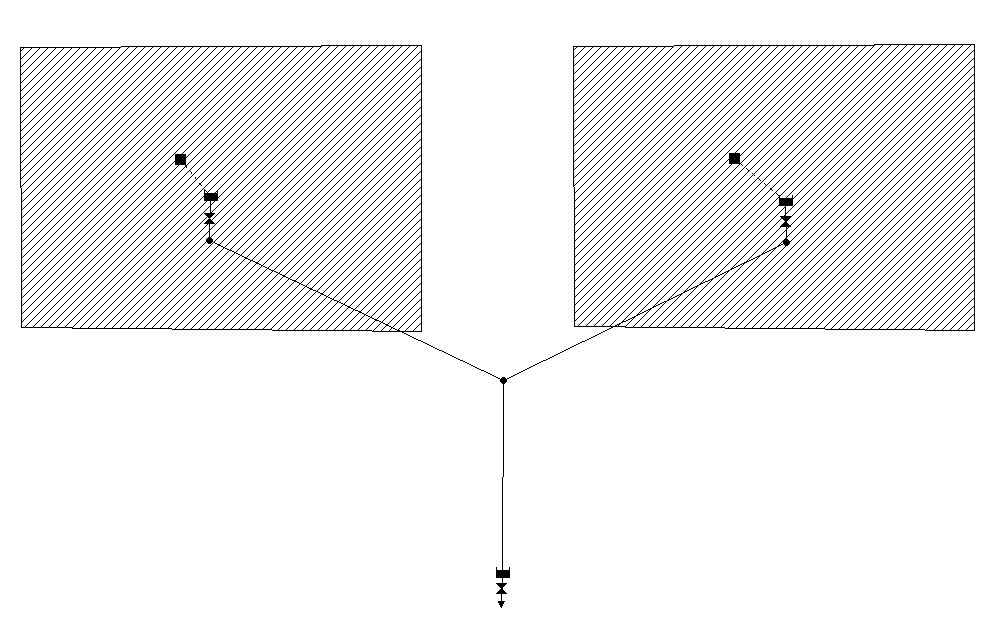
\includegraphics[width = 0.5\textwidth]{Sriesp.JPG}
\end{figure}

\subsection{Site Summary}
\begin{table}[H]
\centering
\label{my-label}
\begin{tabular}{lll}
Element Label & Nature         & Specifications   \\
S1            & Detention Pond & Max Height = 3.6m  \\
  S2            & Detention Pond & Max Height = 3.6m  \\
  S3            & Detention Pond & Max Height = 3.6m  \\
    OR1 & Orifice & Node:S1\\
  OR2 & Orifice & Node:S2 \\
    R3 & Orifice & Node:S3
\end{tabular}
\caption{Table summarizing controllable storm water assets}
\end{table}
[Insert site summary]
\subsection{Uncontrolled Response}
\begin{figure}[H]
  \centering
  \includegraphics[width = 0.9\textwidth]{series_parallel.eps}
\end{figure}

\section{Ann Arbor Network}

\subsection{Network}

\begin{figure}[H]
  \centering
  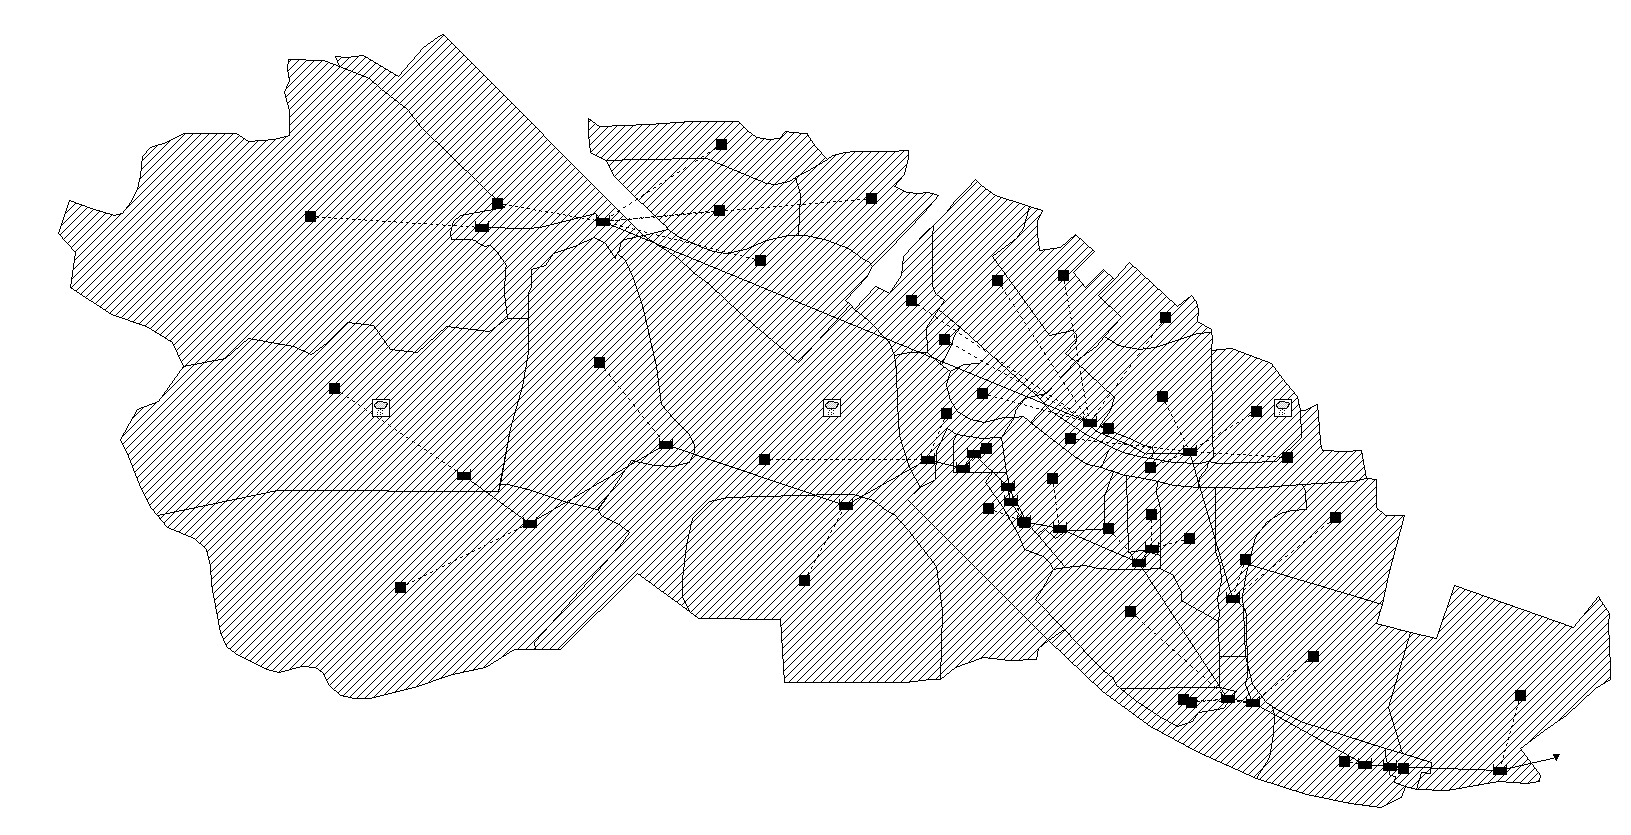
\includegraphics[width = 0.5\textwidth]{Cyndee_Test.PNG}
\end{figure}


\section{Rain Events}

\begin{enumerate}
\item Rainfall - 1
\item Rainfall - 2
\item Rainfall - 3
\end{enumerate} 

\end{document}
